\documentclass[a4paper]{article}

\usepackage[english]{babel}
\usepackage[utf8x]{inputenc}

\usepackage{cite}  % bibliograby
\usepackage{graphicx}  % images
\usepackage{pgfplots}  % plots
  \pgfplotsset{width=10cm,compat=1.9} % plots settings
  \usepgfplotslibrary{external}
  \tikzexternalize



\usepackage{hyperref}  % references
  \hypersetup{colorlinks=true,citecolor=black,filecolor=black,linkcolor=black,urlcolor=black} % references settings

\usepackage[automark]{scrpage2} % heading
  \pagestyle{scrheadings}
  \ihead[]{Handwritten character recognition in MPI} % left header
  \ohead[]{\today} % right header
  \cfoot[]{\pagemark} % footer
  \setheadsepline[122mm]{0.3mm}



\begin{document}
	\title{
	\Huge Handwritten digit recognition
	}
	
	\vspace{2cm}
	
	\author{\Large \href{mailto:stefan.niculae@my.fmi.unibuc.ro}{Stefan Niculae} \and \Large \href{mailto:ionut.ciocoiu@my.fmi.unibuc.ro}{Ionut Ciocoiu}
	\vspace{3cm}}
	
	\date{
	\large Parallel \& Concurrent Programming Lab Report \\
    \vspace{0.2cm}
	\today
	}

	\maketitle
	\setlength{\parindent}{0pt}

\vspace{5cm}
\begin{abstract}
We implement a neural network to classify handwritten digits. The training is done in parallel, using MPI. We provide a comparison for model hyper-parameters and for training time vs number of processes. It achieves great accuracy and fast training time. An interactive demo is also presented
\end{abstract}



\newpage
\tableofcontents



\newpage
\section{Problem statement}
\label{sec:problem}
Given a picture of a handwritten digit, label it accordingly 0 - 9.

\section{Dataset}
\label{sec:dataset}
We demonstrate our model performance on the MNIST database, widely used dataset for training and testing in the field of machine learning. It contains 70 000 examples of labeled handwritten digits. The digits have been size-normalized and centered in a fixed-size image \cite{mnist}. 

\begin{figure}[htb]
\centering

\includegraphics[width=8cm]{images/mnist-images.png}
\caption{Sample MNIST images \cite{tf}}
\end{figure}


The images are black-and-white, with a resolution of $28 \times 28$ pixels, represented as an array of $784$ values. Each value ranges from $0$ to $1$ indicating the amount of blackness in the pixel.

\begin{figure}[htb]
\centering
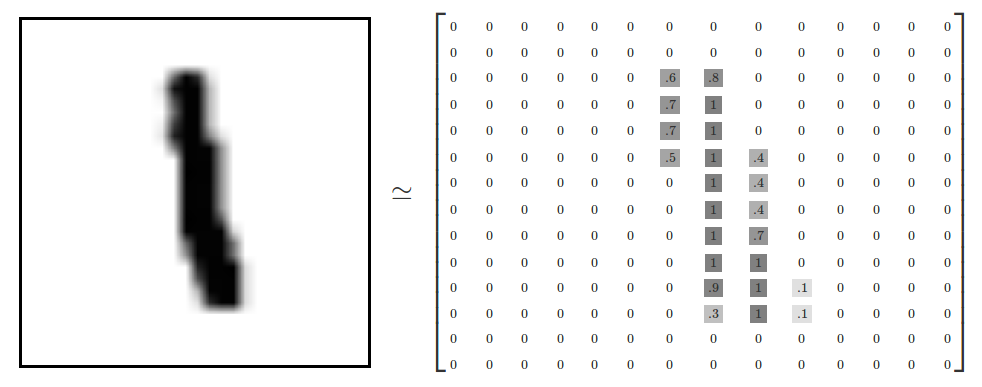
\includegraphics[width=8cm]{images/mnist-matrix.png}
\caption{Matrix representation of a digit \cite{tf}}
\end{figure}


\newpage
\section{Model}
\label{sec:model}
We use a back-propagation neural network with cross-entropy as cost function and soft-max activation. L2 regularization is used to limit overfitting and adaptive learning rate helps soften instability in later epochs.

\begin{figure}[htb]
\centering
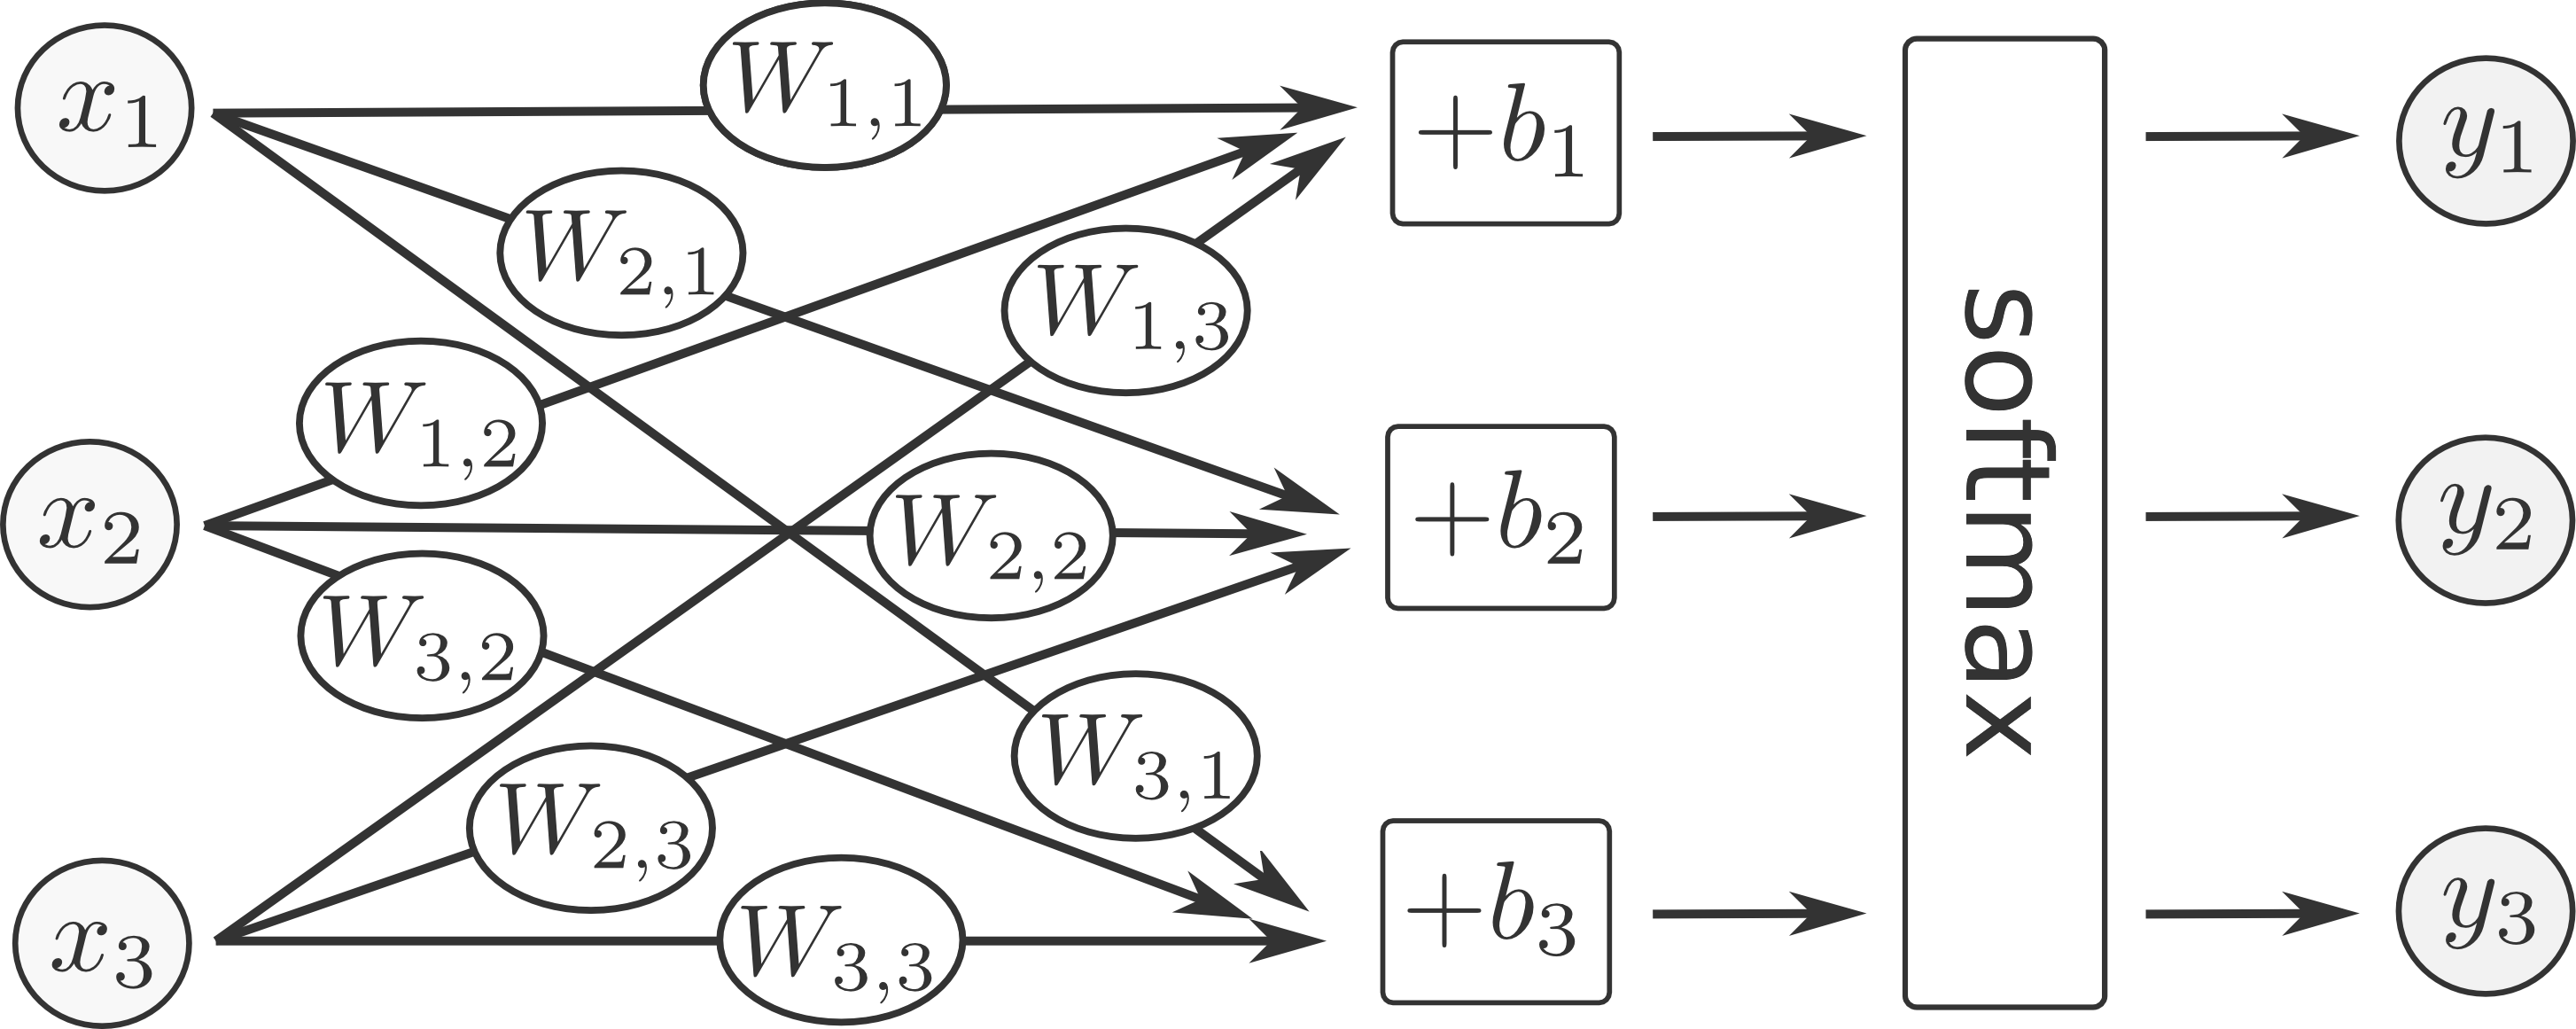
\includegraphics[width=8cm]{images/model-graph.png}
\caption{Simplified representation of model graph \cite{tf}}
\end{figure}

\paragraph{Training} We employ gradient-descent on mini-batches. Early-stopping prevents the model from further learning when performance on the validation split starts decreasing.

\paragraph{Evaluation}
TODO

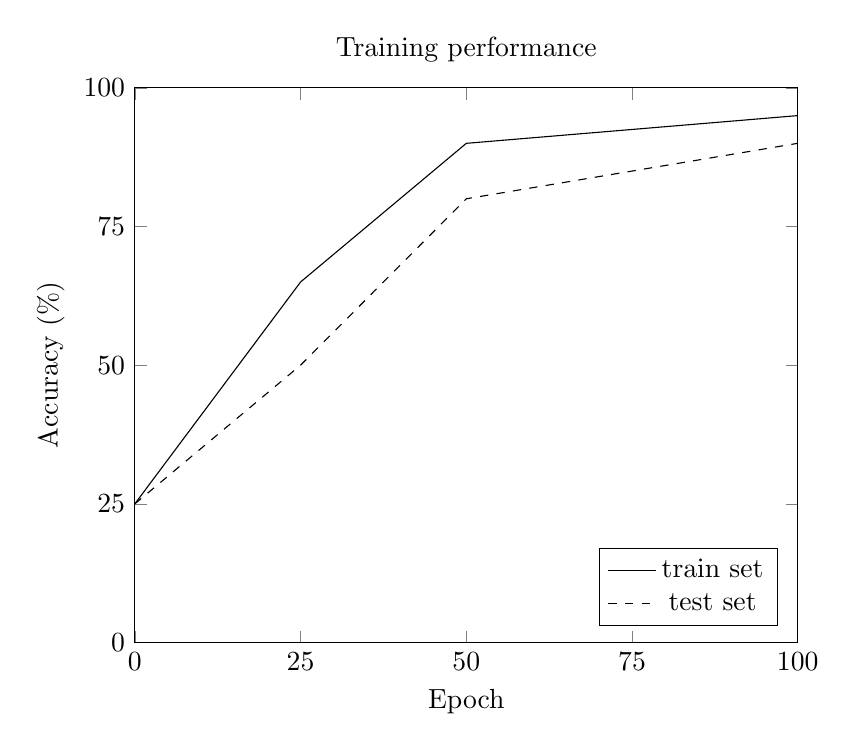
\begin{tikzpicture}
\centering
\begin{axis} [
  title={Training performance},
  xlabel={Epoch},
  ylabel={Accuracy (\%)},
  xmin=0, xmax=100,
  ymin=0, ymax=100,
  xtick={0,25,50,75,100},
  ytick={0,25,50,75,100},
  legend pos=south east,
]

\addplot[]
  coordinates {
  (0,25)(25,65)(50,90)(100,95)
  };
\addplot[dashed]
  coordinates {
  (0,25)(25,50)(50,80)(100,90)
  };
  
\legend{train set, test set}
\end{axis}
\end{tikzpicture}





\newpage
\bibliographystyle{ieeetr}
	\bibliography{references} % expects file "references.bib"
	\addcontentsline{toc}{section}{References}
    
    

\end{document}
